\documentclass{article}
\usepackage{booktabs} % For \toprule, \midrule, and \bottomrule
\usepackage{multirow} % For \multirow
\usepackage{geometry} % For adjusting page dimensions (optional)
\geometry{a4paper, margin=1in} % Adjust margins as needed
\usepackage{pgfplots}
\pgfplotsset{compat=1.18}
\usepackage{siunitx} % For scientific notation
\sisetup{output-exponent-marker=\text{e}} % Optional: to use 'e' notation
\begin{document}
% Updated table code
\begin{table}[htbp]
\centering
\begin{tabular}{@{}ccccc@{}}
\toprule
\multirow{2}{*}{N\_QUBITS} & \multicolumn{2}{c}{TOWER\_CHEBYSHEV} & \multicolumn{2}{c}{FNN\_BASIS} \\
\cmidrule(lr){2-3} \cmidrule(l){4-5}
& Loss & $L_2$ & Loss & $L_2$ \\
\midrule
2 & \num{1.44e1} & \num{2.85e-1} & \num{9.26e-2} & \num{1.14e-2} \\
4 & \num{6.81e-1} & \num{9.29e-2} & \num{5.03e-2} & \num{8.88e-3} \\
6 & \num{5.12e-1} & \num{7.26e-2} & \num{2.90e-2} & \num{5.18e-3} \\
\bottomrule
\end{tabular}
\caption{Comparison of TOWER\_CHEBYSHEV and FNN\_BASIS metrics for different numbers of qubits}
\label{tab:quantum-metrics}
\end{table}
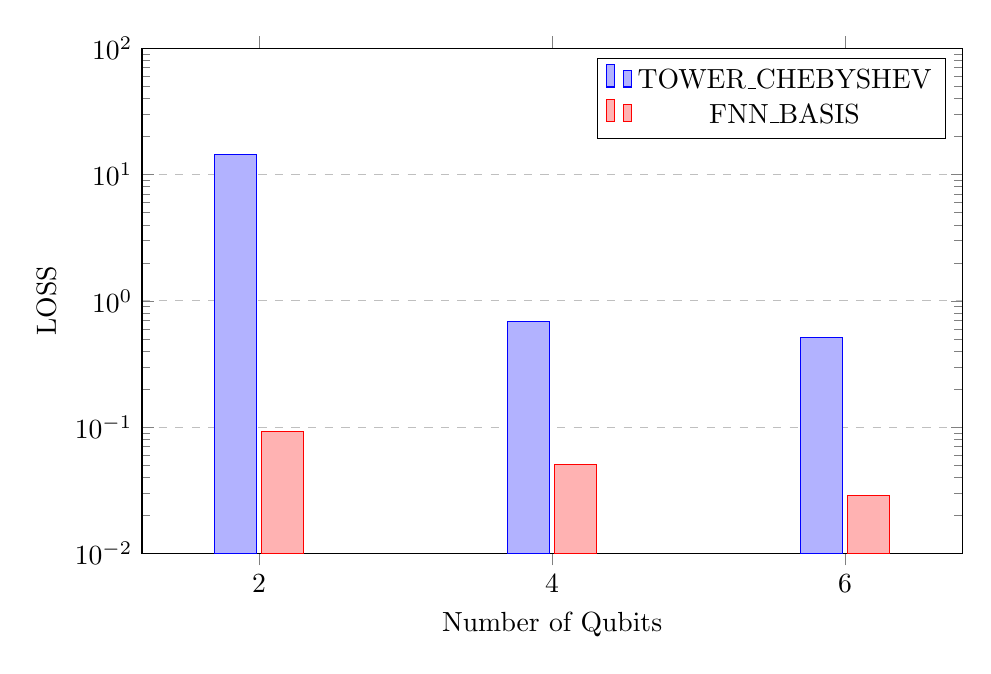
\begin{tikzpicture}
\begin{axis}[
    ybar,
    bar width=15pt,
    width=12cm,
    height=8cm,
    ylabel={LOSS},
    xlabel={Number of Qubits},
    symbolic x coords={2,4,6},
    xtick=data,
    ymode=log,
    log origin=infty,
    ymin=1e-2,
    ymax=100,
    ymajorgrids=true,
    grid style=dashed,
    enlarge x limits=0.2,
    point meta=rawy,
]
\addplot coordinates {(2,14.4) (4,0.681) (6,0.512)};
\addplot coordinates {(2,0.0926) (4,0.0503) (6,0.0290)};
\legend{TOWER\_CHEBYSHEV, FNN\_BASIS}
\end{axis}
\end{tikzpicture}
\end{document}